\documentclass[crop,tikz,convert={outext=.svg,command=\unexpanded{pdf2svg \infile\space\outfile}}]{standalone}

\begin{document}
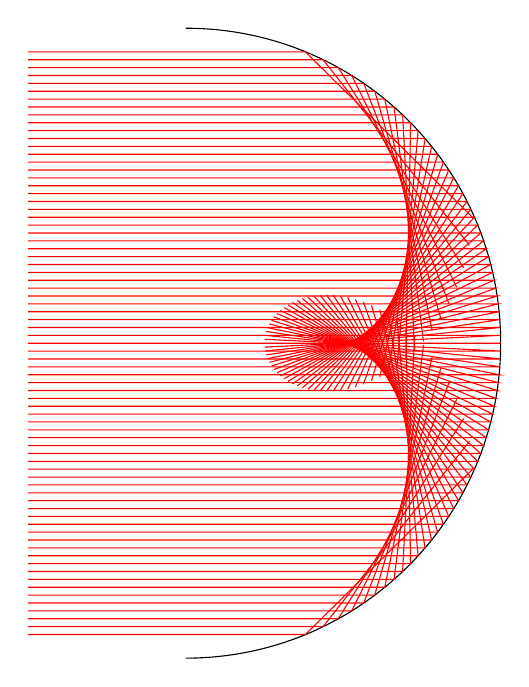
\begin{tikzpicture}
  \pgfmathsetmacro{\radius}{4}
  \draw (-90:\radius) arc (-90:90:\radius);
  \foreach \Y in { -3.7,-3.6,...,3.7 } {%
    \pgfmathsetmacro{\X}{sqrt(\radius*\radius-\Y*\Y)}
    \draw[red] (-\radius/2, \Y) -- ({\X}, \Y) -- +({180+2*atan(\Y/\X)}:3);
  }
\end{tikzpicture}
\end{document}
